\documentclass[12pt]{article}

\usepackage[utf8]{inputenc}
\usepackage[T1]{fontenc}
\usepackage{datetime}
\usepackage[spanish]{babel}
\usepackage{graphicx}
\usepackage{listings}
\usepackage{caption}
\usepackage{subcaption}
\usepackage[right=2cm,left=2cm,top=2cm,bottom=2cm]{geometry}
\usepackage{hyperref}
\usepackage{fancyhdr}
\usepackage{color}
\usepackage[export]{adjustbox}
\usepackage{graphicx}
\usepackage{float}
\usepackage{changepage}
\usepackage{multicol}
\usepackage{imakeidx}
\usepackage{csquotes}
\usepackage{array}
\usepackage{tabularx}
\usepackage{xcolor}
\usepackage[backend=biber]{biblatex}
\addbibresource{webgrafia.bib}

\pagestyle{fancy}
\renewcommand{\footrulewidth}{0.4pt}
\setlength{\headheight}{15pt}


\fancyhead[L]{ CEIABD – SBD }
\fancyhead[R]{ Páez Anguita, Víctor }
\fancyfoot[L]{IES Gran Capitán}


\begin{document}

\begin{titlepage}
    \begin{center}
      \Large \bfseries{}
    \end{center}
    \vspace{0.1cm}
    \begin{center}
      \Large \bfseries{}
    \end{center}
    \vspace{0.1cm}
    \begin{center}
     \Large \bfseries{Análisis Comparativo de Herramientas de Procesamiento de Datos}
    \end{center}
    \vspace{0.0001cm}
    \begin{center}
        Departamento de informática \\ I.E.S. Gran Capitán - Córdoba
    \end{center}
        \vspace{2 cm}
\begin{figure}[h!]
    \centering
    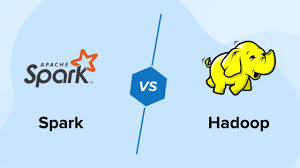
\includegraphics[width=.6\textwidth]{portada.png}
    \label{fig:my_label}
\end{figure}
    \vspace{0.2 cm}
    \begin{center}
        Inteligencia artificial y Big data \\ \currenttime 
    \end{center}
    \vspace{4 cm}
\null\hfill \textbf{Desarrollado por:}
\\
\\
\null\hfill Víctor Páez Anguita
\clearpage
\end{titlepage}

%%%%%%%%%%%%%%%%%%%%%%%%%%%Index%%%%%%%%%%%%%%%%%%%%%%%%%%%%%%%%
\tableofcontents
\clearpage
%%%%%%%%%%%%%%%%%%%%%%%%%%%Index%%%%%%%%%%%%%%%%%%%%%%%%%%%%%%%%

\section{Introducción}



\section{Hadoop}



\subsection{Arquitectura}
\subsection{Ventajas}
\subsection{Desventajas}
\subsection{Aplicaciones}

\subsection{Procesamiento de datos en Hadoop}
\subsubsection{Batch}
\subsubsection{Streaming}
\subsubsection{En tiempo real}


\section{Spark}

\subsection{Arquitectura}
\subsection{Ventajas}
\subsection{Desventajas}
\subsection{Aplicaciones}

\subsection{Procesamiento de datos en Hadoop}
\subsubsection{Batch}
\subsubsection{Streaming}
\subsubsection{En tiempo real}

\section{Comparativa}

\clearpage

\section{Conclusión}


\clearpage

\section{Webgrafia}


Hadoop
\\
Arquitectura
\\
\cite{aprenderbigdata-hadoop}
\cite{ionos-hadoop}
\\
Ventajas y desventajas
\\
\cite{hostzealot-hadoop}
\cite{jacagudelo-hadoop}
\\
Aplicaciones comúnes
\\
\cite{powerdata-hadoop}
\\
Procesamiento de datos en hadoop
\\
\cite{deusto-hadoop}
\\
\\
Spark
\\
Arquitectura
\\
\cite{keepcoding-spark}
\cite{medium-spark}
\\
Ventajas y desventajas
\\
\cite{bbvaapimarket-spark}
\cite{ionos-spark}
\\
Aplicaciones comúnes en Spark
\\
\cite{googleCloud-spark}
\\
Procesamiento de datos en Spark
\\
\cite{diegocalvo-spark}
\\

Comparativa de Hadoop y Spark
\\
\cite{aws-hadoop-spark}
\cite{esic-hadoop-spark}
\cite{inesdi-hadoop-spark}


\printbibliography

\end{document}
